% REV01 Tue 22 Jun 2021 11:28:23 WIB
% START Tue 04 May 2021 13:55:16 WIB

\chapter{MINDERS AND RE-MINDERS}

The Secretary lost no time in getting to work, and his vigilance
and method soon set their mark on the Golden Dustman’s affairs. His
earnestness in determining to understand the length and breadth and
depth of every piece of work submitted to him by his employer, was as
special as his despatch in transacting it. He accepted no information
or explanation at second hand, but made himself the master of everything
confided to him.

One part of the Secretary’s conduct, underlying all the rest, might have
been mistrusted by a man with a better knowledge of men than the
Golden Dustman had. The Secretary was as far from being inquisitive
or intrusive as Secretary could be, but nothing less than a complete
understanding of the whole of the affairs would content him. It soon
became apparent (from the knowledge with which he set out) that he must
have been to the office where the Harmon will was registered, and must
have read the will. He anticipated Mr Boffin’s consideration whether he
should be advised with on this or that topic, by showing that he
already knew of it and understood it. He did this with no attempt at
concealment, seeming to be satisfied that it was part of his duty to
have prepared himself at all attainable points for its utmost discharge.

This might--let it be repeated--have awakened some little vague mistrust
in a man more worldly-wise than the Golden Dustman. On the other hand,
the Secretary was discerning, discreet, and silent, though as zealous as
if the affairs had been his own. He showed no love of patronage or the
command of money, but distinctly preferred resigning both to Mr
Boffin. If, in his limited sphere, he sought power, it was the power
of knowledge; the power derivable from a perfect comprehension of his
business.

As on the Secretary’s face there was a nameless cloud, so on his
manner there was a shadow equally indefinable. It was not that he was
embarrassed, as on that first night with the Wilfer family; he was
habitually unembarrassed now, and yet the something remained. It was not
that his manner was bad, as on that occasion; it was now very good, as
being modest, gracious, and ready. Yet the something never left it. It
has been written of men who have undergone a cruel captivity, or who
have passed through a terrible strait, or who in self-preservation have
killed a defenceless fellow-creature, that the record thereof has never
faded from their countenances until they died. Was there any such record
here?

He established a temporary office for himself in the new house, and all
went well under his hand, with one singular exception. He manifestly
objected to communicate with Mr Boffin’s solicitor. Two or three times,
when there was some slight occasion for his doing so, he transferred
the task to Mr Boffin; and his evasion of it soon became so curiously
apparent, that Mr Boffin spoke to him on the subject of his reluctance.

‘It is so,’ the Secretary admitted. ‘I would rather not.’

Had he any personal objection to Mr Lightwood?

‘I don’t know him.’

Had he suffered from law-suits?

‘Not more than other men,’ was his short answer.

Was he prejudiced against the race of lawyers?

‘No. But while I am in your employment, sir, I would rather be excused
from going between the lawyer and the client. Of course if you press it,
Mr Boffin, I am ready to comply. But I should take it as a great favour
if you would not press it without urgent occasion.’

Now, it could not be said that there WAS urgent occasion, for Lightwood
retained no other affairs in his hands than such as still lingered and
languished about the undiscovered criminal, and such as arose out of the
purchase of the house. Many other matters that might have travelled to
him, now stopped short at the Secretary, under whose administration they
were far more expeditiously and satisfactorily disposed of than they
would have been if they had got into Young Blight’s domain. This the
Golden Dustman quite understood. Even the matter immediately in hand
was of very little moment as requiring personal appearance on the
Secretary’s part, for it amounted to no more than this:--The death of
Hexam rendering the sweat of the honest man’s brow unprofitable, the
honest man had shufflingly declined to moisten his brow for nothing,
with that severe exertion which is known in legal circles as swearing
your way through a stone wall. Consequently, that new light had gone
sputtering out. But, the airing of the old facts had led some one
concerned to suggest that it would be well before they were reconsigned
to their gloomy shelf--now probably for ever--to induce or compel that
Mr Julius Handford to reappear and be questioned. And all traces of Mr
Julius Handford being lost, Lightwood now referred to his client for
authority to seek him through public advertisement.

‘Does your objection go to writing to Lightwood, Rokesmith?’

‘Not in the least, sir.’

‘Then perhaps you’ll write him a line, and say he is free to do what he
likes. I don’t think it promises.’

‘I don’t think it promises,’ said the Secretary.

‘Still, he may do what he likes.’

‘I will write immediately. Let me thank you for so considerately
yielding to my disinclination. It may seem less unreasonable, if I avow
to you that although I don’t know Mr Lightwood, I have a disagreeable
association connected with him. It is not his fault; he is not at all to
blame for it, and does not even know my name.’

Mr Boffin dismissed the matter with a nod or two. The letter was
written, and next day Mr Julius Handford was advertised for. He was
requested to place himself in communication with Mr Mortimer Lightwood,
as a possible means of furthering the ends of justice, and a reward was
offered to any one acquainted with his whereabout who would communicate
the same to the said Mr Mortimer Lightwood at his office in the Temple.
Every day for six weeks this advertisement appeared at the head of all
the newspapers, and every day for six weeks the Secretary, when he
saw it, said to himself; in the tone in which he had said to his
employer,--‘I don’t think it promises!’

Among his first occupations the pursuit of that orphan wanted by
Mrs Boffin held a conspicuous place. From the earliest moment of his
engagement he showed a particular desire to please her, and, knowing her
to have this object at heart, he followed it up with unwearying alacrity
and interest.

Mr and Mrs Milvey had found their search a difficult one. Either an
eligible orphan was of the wrong sex (which almost always happened)
or was too old, or too young, or too sickly, or too dirty, or too much
accustomed to the streets, or too likely to run away; or, it was found
impossible to complete the philanthropic transaction without buying the
orphan. For, the instant it became known that anybody wanted the orphan,
up started some affectionate relative of the orphan who put a price upon
the orphan’s head. The suddenness of an orphan’s rise in the market was
not to be paralleled by the maddest records of the Stock Exchange. He
would be at five thousand per cent discount out at nurse making a mud
pie at nine in the morning, and (being inquired for) would go up to
five thousand per cent premium before noon. The market was ‘rigged’ in
various artful ways. Counterfeit stock got into circulation. Parents
boldly represented themselves as dead, and brought their orphans with
them. Genuine orphan-stock was surreptitiously withdrawn from the
market. It being announced, by emissaries posted for the purpose, that
Mr and Mrs Milvey were coming down the court, orphan scrip would be
instantly concealed, and production refused, save on a condition usually
stated by the brokers as ‘a gallon of beer’. Likewise, fluctuations of
a wild and South-Sea nature were occasioned, by orphan-holders keeping
back, and then rushing into the market a dozen together. But, the
uniform principle at the root of all these various operations was
bargain and sale; and that principle could not be recognized by Mr and
Mrs Milvey.

At length, tidings were received by the Reverend Frank of a charming
orphan to be found at Brentford. One of the deceased parents (late his
parishioners) had a poor widowed grandmother in that agreeable town, and
she, Mrs Betty Higden, had carried off the orphan with maternal care,
but could not afford to keep him.

The Secretary proposed to Mrs Boffin, either to go down himself and
take a preliminary survey of this orphan, or to drive her down, that
she might at once form her own opinion. Mrs Boffin preferring the latter
course, they set off one morning in a hired phaeton, conveying the
hammer-headed young man behind them.

The abode of Mrs Betty Higden was not easy to find, lying in such
complicated back settlements of muddy Brentford that they left their
equipage at the sign of the Three Magpies, and went in search of it on
foot. After many inquiries and defeats, there was pointed out to them
in a lane, a very small cottage residence, with a board across the open
doorway, hooked on to which board by the armpits was a young gentleman
of tender years, angling for mud with a headless wooden horse and line.
In this young sportsman, distinguished by a crisply curling auburn head
and a bluff countenance, the Secretary descried the orphan.

It unfortunately happened as they quickened their pace, that the orphan,
lost to considerations of personal safety in the ardour of the moment,
overbalanced himself and toppled into the street. Being an orphan of a
chubby conformation, he then took to rolling, and had rolled into the
gutter before they could come up. From the gutter he was rescued by John
Rokesmith, and thus the first meeting with Mrs Higden was inaugurated by
the awkward circumstance of their being in possession--one would say at
first sight unlawful possession--of the orphan, upside down and purple
in the countenance. The board across the doorway too, acting as a trap
equally for the feet of Mrs Higden coming out, and the feet of Mrs
Boffin and John Rokesmith going in, greatly increased the difficulty of
the situation: to which the cries of the orphan imparted a lugubrious
and inhuman character.

At first, it was impossible to explain, on account of the orphan’s
‘holding his breath’: a most terrific proceeding, super-inducing in the
orphan lead-colour rigidity and a deadly silence, compared with which
his cries were music yielding the height of enjoyment. But as he
gradually recovered, Mrs Boffin gradually introduced herself; and
smiling peace was gradually wooed back to Mrs Betty Higden’s home.

It was then perceived to be a small home with a large mangle in it, at
the handle of which machine stood a very long boy, with a very little
head, and an open mouth of disproportionate capacity that seemed to
assist his eyes in staring at the visitors. In a corner below the
mangle, on a couple of stools, sat two very little children: a boy and a
girl; and when the very long boy, in an interval of staring, took a turn
at the mangle, it was alarming to see how it lunged itself at those two
innocents, like a catapult designed for their destruction, harmlessly
retiring when within an inch of their heads. The room was clean and
neat. It had a brick floor, and a window of diamond panes, and a flounce
hanging below the chimney-piece, and strings nailed from bottom to top
outside the window on which scarlet-beans were to grow in the coming
season if the Fates were propitious. However propitious they might have
been in the seasons that were gone, to Betty Higden in the matter of
beans, they had not been very favourable in the matter of coins; for it
was easy to see that she was poor.

She was one of those old women, was Mrs Betty Higden, who by dint of
an indomitable purpose and a strong constitution fight out many years,
though each year has come with its new knock-down blows fresh to the
fight against her, wearied by it; an active old woman, with a bright
dark eye and a resolute face, yet quite a tender creature too; not a
logically-reasoning woman, but God is good, and hearts may count in
Heaven as high as heads.

‘Yes sure!’ said she, when the business was opened, ‘Mrs Milvey had the
kindness to write to me, ma’am, and I got Sloppy to read it. It was a
pretty letter. But she’s an affable lady.’

The visitors glanced at the long boy, who seemed to indicate by a
broader stare of his mouth and eyes that in him Sloppy stood confessed.

‘For I aint, you must know,’ said Betty, ‘much of a hand at reading
writing-hand, though I can read my Bible and most print. And I do love a
newspaper. You mightn’t think it, but Sloppy is a beautiful reader of a
newspaper. He do the Police in different voices.’

The visitors again considered it a point of politeness to look at
Sloppy, who, looking at them, suddenly threw back his head, extended his
mouth to its utmost width, and laughed loud and long. At this the two
innocents, with their brains in that apparent danger, laughed, and Mrs
Higden laughed, and the orphan laughed, and then the visitors laughed.
Which was more cheerful than intelligible.

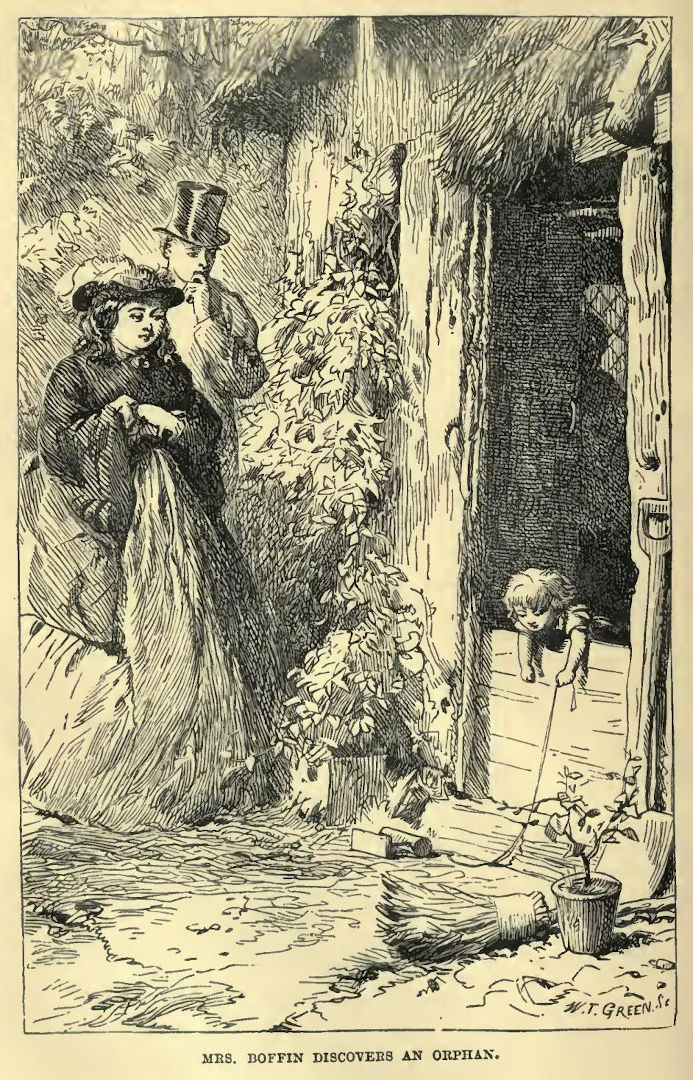
\includegraphics[scale=2.3]{01-16-01}

Then Sloppy seeming to be seized with an industrious mania or fury,
turned to at the mangle, and impelled it at the heads of the innocents
with such a creaking and rumbling, that Mrs Higden stopped him.

‘The gentlefolks can’t hear themselves speak, Sloppy. Bide a bit, bide a
bit!’

‘Is that the dear child in your lap?’ said Mrs Boffin.

‘Yes, ma’am, this is Johnny.’

‘Johnny, too!’ cried Mrs Boffin, turning to the Secretary; ‘already
Johnny! Only one of the two names left to give him! He’s a pretty boy.’

With his chin tucked down in his shy childish manner, he was looking
furtively at Mrs Boffin out of his blue eyes, and reaching his fat
dimpled hand up to the lips of the old woman, who was kissing it by
times.

‘Yes, ma’am, he’s a pretty boy, he’s a dear darling boy, he’s the child
of my own last left daughter’s daughter. But she’s gone the way of all
the rest.’

‘Those are not his brother and sister?’ said Mrs Boffin.

‘Oh, dear no, ma’am. Those are Minders.’

‘Minders?’ the Secretary repeated.

‘Left to be Minded, sir. I keep a Minding-School. I can take only three,
on account of the Mangle. But I love children, and Four-pence a week is
Four-pence. Come here, Toddles and Poddles.’

Toddles was the pet-name of the boy; Poddles of the girl. At their
little unsteady pace, they came across the floor, hand-in-hand, as if
they were traversing an extremely difficult road intersected by brooks,
and, when they had had their heads patted by Mrs Betty Higden, made
lunges at the orphan, dramatically representing an attempt to bear him,
crowing, into captivity and slavery. All the three children enjoyed this
to a delightful extent, and the sympathetic Sloppy again laughed long
and loud. When it was discreet to stop the play, Betty Higden said
‘Go to your seats Toddles and Poddles,’ and they returned hand-in-hand
across country, seeming to find the brooks rather swollen by late rains.

‘And Master--or Mister--Sloppy?’ said the Secretary, in doubt whether he
was man, boy, or what.

‘A love-child,’ returned Betty Higden, dropping her voice; ‘parents
never known; found in the street. He was brought up in the--’ with a
shiver of repugnance, ‘--the House.’

‘The Poor-house?’ said the Secretary.

Mrs Higden set that resolute old face of hers, and darkly nodded yes.

‘You dislike the mention of it.’

‘Dislike the mention of it?’ answered the old woman. ‘Kill me sooner
than take me there. Throw this pretty child under cart-horses feet and
a loaded waggon, sooner than take him there. Come to us and find us all
a-dying, and set a light to us all where we lie and let us all blaze
away with the house into a heap of cinders sooner than move a corpse of
us there!’

A surprising spirit in this lonely woman after so many years of hard
working, and hard living, my Lords and Gentlemen and Honourable
Boards! What is it that we call it in our grandiose speeches? British
independence, rather perverted? Is that, or something like it, the ring
of the cant?

‘Do I never read in the newspapers,’ said the dame, fondling the
child--‘God help me and the like of me!--how the worn-out people that
do come down to that, get driven from post to pillar and pillar to post,
a-purpose to tire them out! Do I never read how they are put off, put
off, put off--how they are grudged, grudged, grudged, the shelter, or
the doctor, or the drop of physic, or the bit of bread? Do I never
read how they grow heartsick of it and give it up, after having let
themselves drop so low, and how they after all die out for want of help?
Then I say, I hope I can die as well as another, and I’ll die without
that disgrace.’

Absolutely impossible my Lords and Gentlemen and Honourable Boards, by
any stretch of legislative wisdom to set these perverse people right in
their logic?

‘Johnny, my pretty,’ continued old Betty, caressing the child, and
rather mourning over it than speaking to it, ‘your old Granny Betty is
nigher fourscore year than threescore and ten. She never begged nor had
a penny of the Union money in all her life. She paid scot and she
paid lot when she had money to pay; she worked when she could, and
she starved when she must. You pray that your Granny may have strength
enough left her at the last (she’s strong for an old one, Johnny), to
get up from her bed and run and hide herself and swown to death in a
hole, sooner than fall into the hands of those Cruel Jacks we read of
that dodge and drive, and worry and weary, and scorn and shame, the
decent poor.’

A brilliant success, my Lords and Gentlemen and Honourable Boards to
have brought it to this in the minds of the best of the poor! Under
submission, might it be worth thinking of at any odd time?

The fright and abhorrence that Mrs Betty Higden smoothed out of her
strong face as she ended this diversion, showed how seriously she had
meant it.

‘And does he work for you?’ asked the Secretary, gently bringing the
discourse back to Master or Mister Sloppy.

‘Yes,’ said Betty with a good-humoured smile and nod of the head. ‘And
well too.’

‘Does he live here?’

‘He lives more here than anywhere. He was thought to be no better than a
Natural, and first come to me as a Minder. I made interest with Mr Blogg
the Beadle to have him as a Minder, seeing him by chance up at church,
and thinking I might do something with him. For he was a weak ricketty
creetur then.’

‘Is he called by his right name?’

‘Why, you see, speaking quite correctly, he has no right name. I always
understood he took his name from being found on a Sloppy night.’

‘He seems an amiable fellow.’

‘Bless you, sir, there’s not a bit of him,’ returned Betty, ‘that’s not
amiable. So you may judge how amiable he is, by running your eye along
his heighth.’

Of an ungainly make was Sloppy. Too much of him longwise, too little of
him broadwise, and too many sharp angles of him angle-wise. One of those
shambling male human creatures, born to be indiscreetly candid in the
revelation of buttons; every button he had about him glaring at the
public to a quite preternatural extent. A considerable capital of knee
and elbow and wrist and ankle, had Sloppy, and he didn’t know how to
dispose of it to the best advantage, but was always investing it in
wrong securities, and so getting himself into embarrassed circumstances.
Full-Private Number One in the Awkward Squad of the rank and file of
life, was Sloppy, and yet had his glimmering notions of standing true to
the Colours.

‘And now,’ said Mrs Boffin, ‘concerning Johnny.’

As Johnny, with his chin tucked in and lips pouting, reclined in Betty’s
lap, concentrating his blue eyes on the visitors and shading them from
observation with a dimpled arm, old Betty took one of his fresh fat
hands in her withered right, and fell to gently beating it on her
withered left.

‘Yes, ma’am. Concerning Johnny.’

‘If you trust the dear child to me,’ said Mrs Boffin, with a face
inviting trust, ‘he shall have the best of homes, the best of care, the
best of education, the best of friends. Please God I will be a true good
mother to him!’

‘I am thankful to you, ma’am, and the dear child would be thankful if
he was old enough to understand.’ Still lightly beating the little hand
upon her own. ‘I wouldn’t stand in the dear child’s light, not if I had
all my life before me instead of a very little of it. But I hope you
won’t take it ill that I cleave to the child closer than words can tell,
for he’s the last living thing left me.’

‘Take it ill, my dear soul? Is it likely? And you so tender of him as to
bring him home here!’

‘I have seen,’ said Betty, still with that light beat upon her hard
rough hand, ‘so many of them on my lap. And they are all gone but this
one! I am ashamed to seem so selfish, but I don’t really mean it. It’ll
be the making of his fortune, and he’ll be a gentleman when I am dead.
I--I--don’t know what comes over me. I--try against it. Don’t notice
me!’ The light beat stopped, the resolute mouth gave way, and the fine
strong old face broke up into weakness and tears.

Now, greatly to the relief of the visitors, the emotional Sloppy no
sooner beheld his patroness in this condition, than, throwing back his
head and throwing open his mouth, he lifted up his voice and bellowed.
This alarming note of something wrong instantly terrified Toddles and
Poddles, who were no sooner heard to roar surprisingly, than Johnny,
curving himself the wrong way and striking out at Mrs Boffin with a pair
of indifferent shoes, became a prey to despair. The absurdity of the
situation put its pathos to the rout. Mrs Betty Higden was herself in
a moment, and brought them all to order with that speed, that Sloppy,
stopping short in a polysyllabic bellow, transferred his energy to
the mangle, and had taken several penitential turns before he could be
stopped.

‘There, there, there!’ said Mrs Boffin, almost regarding her kind self
as the most ruthless of women. ‘Nothing is going to be done. Nobody need
be frightened. We’re all comfortable; ain’t we, Mrs Higden?’

‘Sure and certain we are,’ returned Betty.

‘And there really is no hurry, you know,’ said Mrs Boffin in a lower
voice. ‘Take time to think of it, my good creature!’

‘Don’t you fear ME no more, ma’am,’ said Betty; ‘I thought of it for
good yesterday. I don’t know what come over me just now, but it’ll never
come again.’

‘Well, then, Johnny shall have more time to think of it,’ returned Mrs
Boffin; ‘the pretty child shall have time to get used to it. And you’ll
get him more used to it, if you think well of it; won’t you?’

Betty undertook that, cheerfully and readily.

‘Lor,’ cried Mrs Boffin, looking radiantly about her, ‘we want to make
everybody happy, not dismal!--And perhaps you wouldn’t mind letting me
know how used to it you begin to get, and how it all goes on?’

‘I’ll send Sloppy,’ said Mrs Higden.

‘And this gentleman who has come with me will pay him for his trouble,’
said Mrs Boffin. ‘And Mr Sloppy, whenever you come to my house, be
sure you never go away without having had a good dinner of meat, beer,
vegetables, and pudding.’

This still further brightened the face of affairs; for, the highly
sympathetic Sloppy, first broadly staring and grinning, and then roaring
with laughter, Toddles and Poddles followed suit, and Johnny trumped
the trick. T and P considering these favourable circumstances for
the resumption of that dramatic descent upon Johnny, again came
across-country hand-in-hand upon a buccaneering expedition; and this
having been fought out in the chimney corner behind Mrs Higden’s chair,
with great valour on both sides, those desperate pirates returned
hand-in-hand to their stools, across the dry bed of a mountain torrent.

‘You must tell me what I can do for you, Betty my friend,’ said Mrs
Boffin confidentially, ‘if not to-day, next time.’

‘Thank you all the same, ma’am, but I want nothing for myself. I can
work. I’m strong. I can walk twenty mile if I’m put to it.’ Old Betty
was proud, and said it with a sparkle in her bright eyes.

‘Yes, but there are some little comforts that you wouldn’t be the worse
for,’ returned Mrs Boffin. ‘Bless ye, I wasn’t born a lady any more than
you.’

‘It seems to me,’ said Betty, smiling, ‘that you were born a lady, and
a true one, or there never was a lady born. But I couldn’t take anything
from you, my dear. I never did take anything from any one. It ain’t that
I’m not grateful, but I love to earn it better.’

‘Well, well!’ returned Mrs Boffin. ‘I only spoke of little things, or I
wouldn’t have taken the liberty.’

Betty put her visitor’s hand to her lips, in acknowledgment of the
delicate answer. Wonderfully upright her figure was, and wonderfully
self-reliant her look, as, standing facing her visitor, she explained
herself further.

‘If I could have kept the dear child, without the dread that’s always
upon me of his coming to that fate I have spoken of, I could never have
parted with him, even to you. For I love him, I love him, I love him! I
love my husband long dead and gone, in him; I love my children dead and
gone, in him; I love my young and hopeful days dead and gone, in him. I
couldn’t sell that love, and look you in your bright kind face. It’s a
free gift. I am in want of nothing. When my strength fails me, if I
can but die out quick and quiet, I shall be quite content. I have stood
between my dead and that shame I have spoken of; and it has been kept
off from every one of them. Sewed into my gown,’ with her hand upon
her breast, ‘is just enough to lay me in the grave. Only see that it’s
rightly spent, so as I may rest free to the last from that cruelty and
disgrace, and you’ll have done much more than a little thing for me, and
all that in this present world my heart is set upon.’

Mrs Betty Higden’s visitor pressed her hand. There was no more breaking
up of the strong old face into weakness. My Lords and Gentlemen and
Honourable Boards, it really was as composed as our own faces, and
almost as dignified.

And now, Johnny was to be inveigled into occupying a temporary
position on Mrs Boffin’s lap. It was not until he had been piqued into
competition with the two diminutive Minders, by seeing them successively
raised to that post and retire from it without injury, that he could be
by any means induced to leave Mrs Betty Higden’s skirts; towards which
he exhibited, even when in Mrs Boffin’s embrace, strong yearnings,
spiritual and bodily; the former expressed in a very gloomy visage,
the latter in extended arms. However, a general description of the
toy-wonders lurking in Mr Boffin’s house, so far conciliated this
worldly-minded orphan as to induce him to stare at her frowningly,
with a fist in his mouth, and even at length to chuckle when a
richly-caparisoned horse on wheels, with a miraculous gift of cantering
to cake-shops, was mentioned. This sound being taken up by the Minders,
swelled into a rapturous trio which gave general satisfaction.

So, the interview was considered very successful, and Mrs Boffin was
pleased, and all were satisfied. Not least of all, Sloppy, who undertook
to conduct the visitors back by the best way to the Three Magpies, and
whom the hammer-headed young man much despised.

This piece of business thus put in train, the Secretary drove Mrs Boffin
back to the Bower, and found employment for himself at the new house
until evening. Whether, when evening came, he took a way to his lodgings
that led through fields, with any design of finding Miss Bella Wilfer
in those fields, is not so certain as that she regularly walked there at
that hour.

And, moreover, it is certain that there she was.

No longer in mourning, Miss Bella was dressed in as pretty colours as
she could muster. There is no denying that she was as pretty as they,
and that she and the colours went very prettily together. She was
reading as she walked, and of course it is to be inferred, from her
showing no knowledge of Mr Rokesmith’s approach, that she did not know
he was approaching.

‘Eh?’ said Miss Bella, raising her eyes from her book, when he stopped
before her. ‘Oh! It’s you.’

‘Only I. A fine evening!’

‘Is it?’ said Bella, looking coldly round. ‘I suppose it is, now you
mention it. I have not been thinking of the evening.’

‘So intent upon your book?’

‘Ye-e-es,’ replied Bella, with a drawl of indifference.

‘A love story, Miss Wilfer?’

‘Oh dear no, or I shouldn’t be reading it. It’s more about money than
anything else.’

‘And does it say that money is better than anything?’

‘Upon my word,’ returned Bella, ‘I forget what it says, but you can find
out for yourself if you like, Mr Rokesmith. I don’t want it any more.’

The Secretary took the book--she had fluttered the leaves as if it were
a fan--and walked beside her.

‘I am charged with a message for you, Miss Wilfer.’

‘Impossible, I think!’ said Bella, with another drawl.

‘From Mrs Boffin. She desired me to assure you of the pleasure she has
in finding that she will be ready to receive you in another week or two
at furthest.’

Bella turned her head towards him, with her prettily-insolent eyebrows
raised, and her eyelids drooping. As much as to say, ‘How did YOU come
by the message, pray?’

‘I have been waiting for an opportunity of telling you that I am Mr
Boffin’s Secretary.’

‘I am as wise as ever,’ said Miss Bella, loftily, ‘for I don’t know what
a Secretary is. Not that it signifies.’

‘Not at all.’

A covert glance at her face, as he walked beside her, showed him that
she had not expected his ready assent to that proposition.

‘Then are you going to be always there, Mr Rokesmith?’ she inquired, as
if that would be a drawback.

‘Always? No. Very much there? Yes.’

‘Dear me!’ drawled Bella, in a tone of mortification.

‘But my position there as Secretary, will be very different from yours
as guest. You will know little or nothing about me. I shall transact
the business: you will transact the pleasure. I shall have my salary to
earn; you will have nothing to do but to enjoy and attract.’

‘Attract, sir?’ said Bella, again with her eyebrows raised, and her
eyelids drooping. ‘I don’t understand you.’

Without replying on this point, Mr Rokesmith went on.

‘Excuse me; when I first saw you in your black dress--’

[‘There!’ was Miss Bella’s mental exclamation. ‘What did I say to them
at home? Everybody noticed that ridiculous mourning.’)

‘When I first saw you in your black dress, I was at a loss to account
for that distinction between yourself and your family. I hope it was not
impertinent to speculate upon it?’

‘I hope not, I am sure,’ said Miss Bella, haughtily. ‘But you ought to
know best how you speculated upon it.’

Mr Rokesmith inclined his head in a deprecatory manner, and went on.

‘Since I have been entrusted with Mr Boffin’s affairs, I have
necessarily come to understand the little mystery. I venture to remark
that I feel persuaded that much of your loss may be repaired. I
speak, of course, merely of wealth, Miss Wilfer. The loss of a perfect
stranger, whose worth, or worthlessness, I cannot estimate--nor you
either--is beside the question. But this excellent gentleman and lady
are so full of simplicity, so full of generosity, so inclined towards
you, and so desirous to--how shall I express it?--to make amends for
their good fortune, that you have only to respond.’

As he watched her with another covert look, he saw a certain ambitious
triumph in her face which no assumed coldness could conceal.

‘As we have been brought under one roof by an accidental combination of
circumstances, which oddly extends itself to the new relations before
us, I have taken the liberty of saying these few words. You don’t
consider them intrusive I hope?’ said the Secretary with deference.

‘Really, Mr Rokesmith, I can’t say what I consider them,’ returned the
young lady. ‘They are perfectly new to me, and may be founded altogether
on your own imagination.’

‘You will see.’

These same fields were opposite the Wilfer premises. The discreet
Mrs Wilfer now looking out of window and beholding her daughter in
conference with her lodger, instantly tied up her head and came out for
a casual walk.

‘I have been telling Miss Wilfer,’ said John Rokesmith, as the majestic
lady came stalking up, ‘that I have become, by a curious chance, Mr
Boffin’s Secretary or man of business.’

‘I have not,’ returned Mrs Wilfer, waving her gloves in her chronic
state of dignity, and vague ill-usage, ‘the honour of any intimate
acquaintance with Mr Boffin, and it is not for me to congratulate that
gentleman on the acquisition he has made.’

‘A poor one enough,’ said Rokesmith.

‘Pardon me,’ returned Mrs Wilfer, ‘the merits of Mr Boffin may be highly
distinguished--may be more distinguished than the countenance of Mrs
Boffin would imply--but it were the insanity of humility to deem him
worthy of a better assistant.’

‘You are very good. I have also been telling Miss Wilfer that she is
expected very shortly at the new residence in town.’

‘Having tacitly consented,’ said Mrs Wilfer, with a grand shrug of her
shoulders, and another wave of her gloves, ‘to my child’s acceptance of
the proffered attentions of Mrs Boffin, I interpose no objection.’

Here Miss Bella offered the remonstrance: ‘Don’t talk nonsense, ma,
please.’

‘Peace!’ said Mrs Wilfer.

‘No, ma, I am not going to be made so absurd. Interposing objections!’

‘I say,’ repeated Mrs Wilfer, with a vast access of grandeur, ‘that I am
NOT going to interpose objections. If Mrs Boffin (to whose countenance
no disciple of Lavater could possibly for a single moment subscribe),’
with a shiver, ‘seeks to illuminate her new residence in town with the
attractions of a child of mine, I am content that she should be favoured
by the company of a child of mine.’

‘You use the word, ma’am, I have myself used,’ said Rokesmith, with a
glance at Bella, ‘when you speak of Miss Wilfer’s attractions there.’

‘Pardon me,’ returned Mrs Wilfer, with dreadful solemnity, ‘but I had
not finished.’

‘Pray excuse me.’

‘I was about to say,’ pursued Mrs Wilfer, who clearly had not had
the faintest idea of saying anything more: ‘that when I use the term
attractions, I do so with the qualification that I do not mean it in any
way whatever.’

The excellent lady delivered this luminous elucidation of her views
with an air of greatly obliging her hearers, and greatly distinguishing
herself. Whereat Miss Bella laughed a scornful little laugh and said:

‘Quite enough about this, I am sure, on all sides. Have the goodness, Mr
Rokesmith, to give my love to Mrs Boffin--’

‘Pardon me!’ cried Mrs Wilfer. ‘Compliments.’

‘Love!’ repeated Bella, with a little stamp of her foot.

‘No!’ said Mrs Wilfer, monotonously. ‘Compliments.’

(‘Say Miss Wilfer’s love, and Mrs Wilfer’s compliments,’ the Secretary
proposed, as a compromise.)

‘And I shall be very glad to come when she is ready for me. The sooner,
the better.’

‘One last word, Bella,’ said Mrs Wilfer, ‘before descending to the
family apartment. I trust that as a child of mine you will ever be
sensible that it will be graceful in you, when associating with Mr
and Mrs Boffin upon equal terms, to remember that the Secretary, Mr
Rokesmith, as your father’s lodger, has a claim on your good word.’

The condescension with which Mrs Wilfer delivered this proclamation of
patronage, was as wonderful as the swiftness with which the lodger
had lost caste in the Secretary. He smiled as the mother retired down
stairs; but his face fell, as the daughter followed.

‘So insolent, so trivial, so capricious, so mercenary, so careless, so
hard to touch, so hard to turn!’ he said, bitterly.

And added as he went upstairs. ‘And yet so pretty, so pretty!’

And added presently, as he walked to and fro in his room. ‘And if she
knew!’

She knew that he was shaking the house by his walking to and fro; and
she declared it another of the miseries of being poor, that you couldn’t
get rid of a haunting Secretary, stump--stump--stumping overhead in the
dark, like a Ghost.



